% LaTeX Template for short student reports.
% Citations should be in bibtex format and go in references.bib
\documentclass[a4paper, 11pt]{article}
\usepackage[top=3cm, bottom=3cm, left = 2cm, right = 2cm]{geometry} 
\geometry{a4paper} 
\usepackage[utf8]{inputenc}
\usepackage{textcomp}
\usepackage{graphicx} 
\usepackage{amsmath,amssymb}  
\usepackage{bm}  
\usepackage[pdftex,bookmarks,colorlinks,breaklinks]{hyperref}  
\hypersetup{linkcolor=black,citecolor=black,filecolor=black,urlcolor=black} % black links, for printed output
\usepackage{memhfixc} 
\usepackage{pdfsync}  
\usepackage{fancyhdr}
\usepackage{fancyvrb}
\usepackage{natbib}
\usepackage{url}
%\pagestyle{fancy}
\usepackage{tabto}
\usepackage[shortlabels]{enumitem}
\usepackage{tikz}
\usepackage{verbatim}
\usepackage{nameref}
\usepackage{caption}
\usepackage{subcaption}
\usepackage{mathtools}

\title{Untitled: A DirectX Game}
\author{Sam Drysdale}
\date{May 16, 2023}

\begin{document}
\graphicspath{{./Images/}}
\maketitle
\tableofcontents
\begin{flushleft}

\section{Summary}

\textit{Untitled} is [...].

\section{User Controls}


\section{Features}\label{Features}

The following is a technical discussion of the key features of \textit{Untitled}, with a focus on advanced procedural generation. Mathematical models and code snippets are kept to a minimum, edited for clarity rather than accuracy to the original application.

\subsection{Noise} % TECHNIQUE: Perlin/simplex noise...

\subsection{Procedural Terrain} % TECHNIQUE: Marching cubes...

Given its grounding in nuclear semiotics, this game's terrain is of course intended to evoke a sense of ``shunned land'' \citep{trth93}. In generating the jutting thorns and blocks so essential to the post-nuclear setting, though, there comes a problem - concavity. Height maps are perfectly adequate for creating rolling hills and valleys, but the fact that each $(x,z)$-coordinate can correspond to only one $y$-value prevents any features that ominously overhang \textit{Untitled}'s barren earth (see Figure \ref{Concave Terrain}).

\begin{figure}[h]
\centering
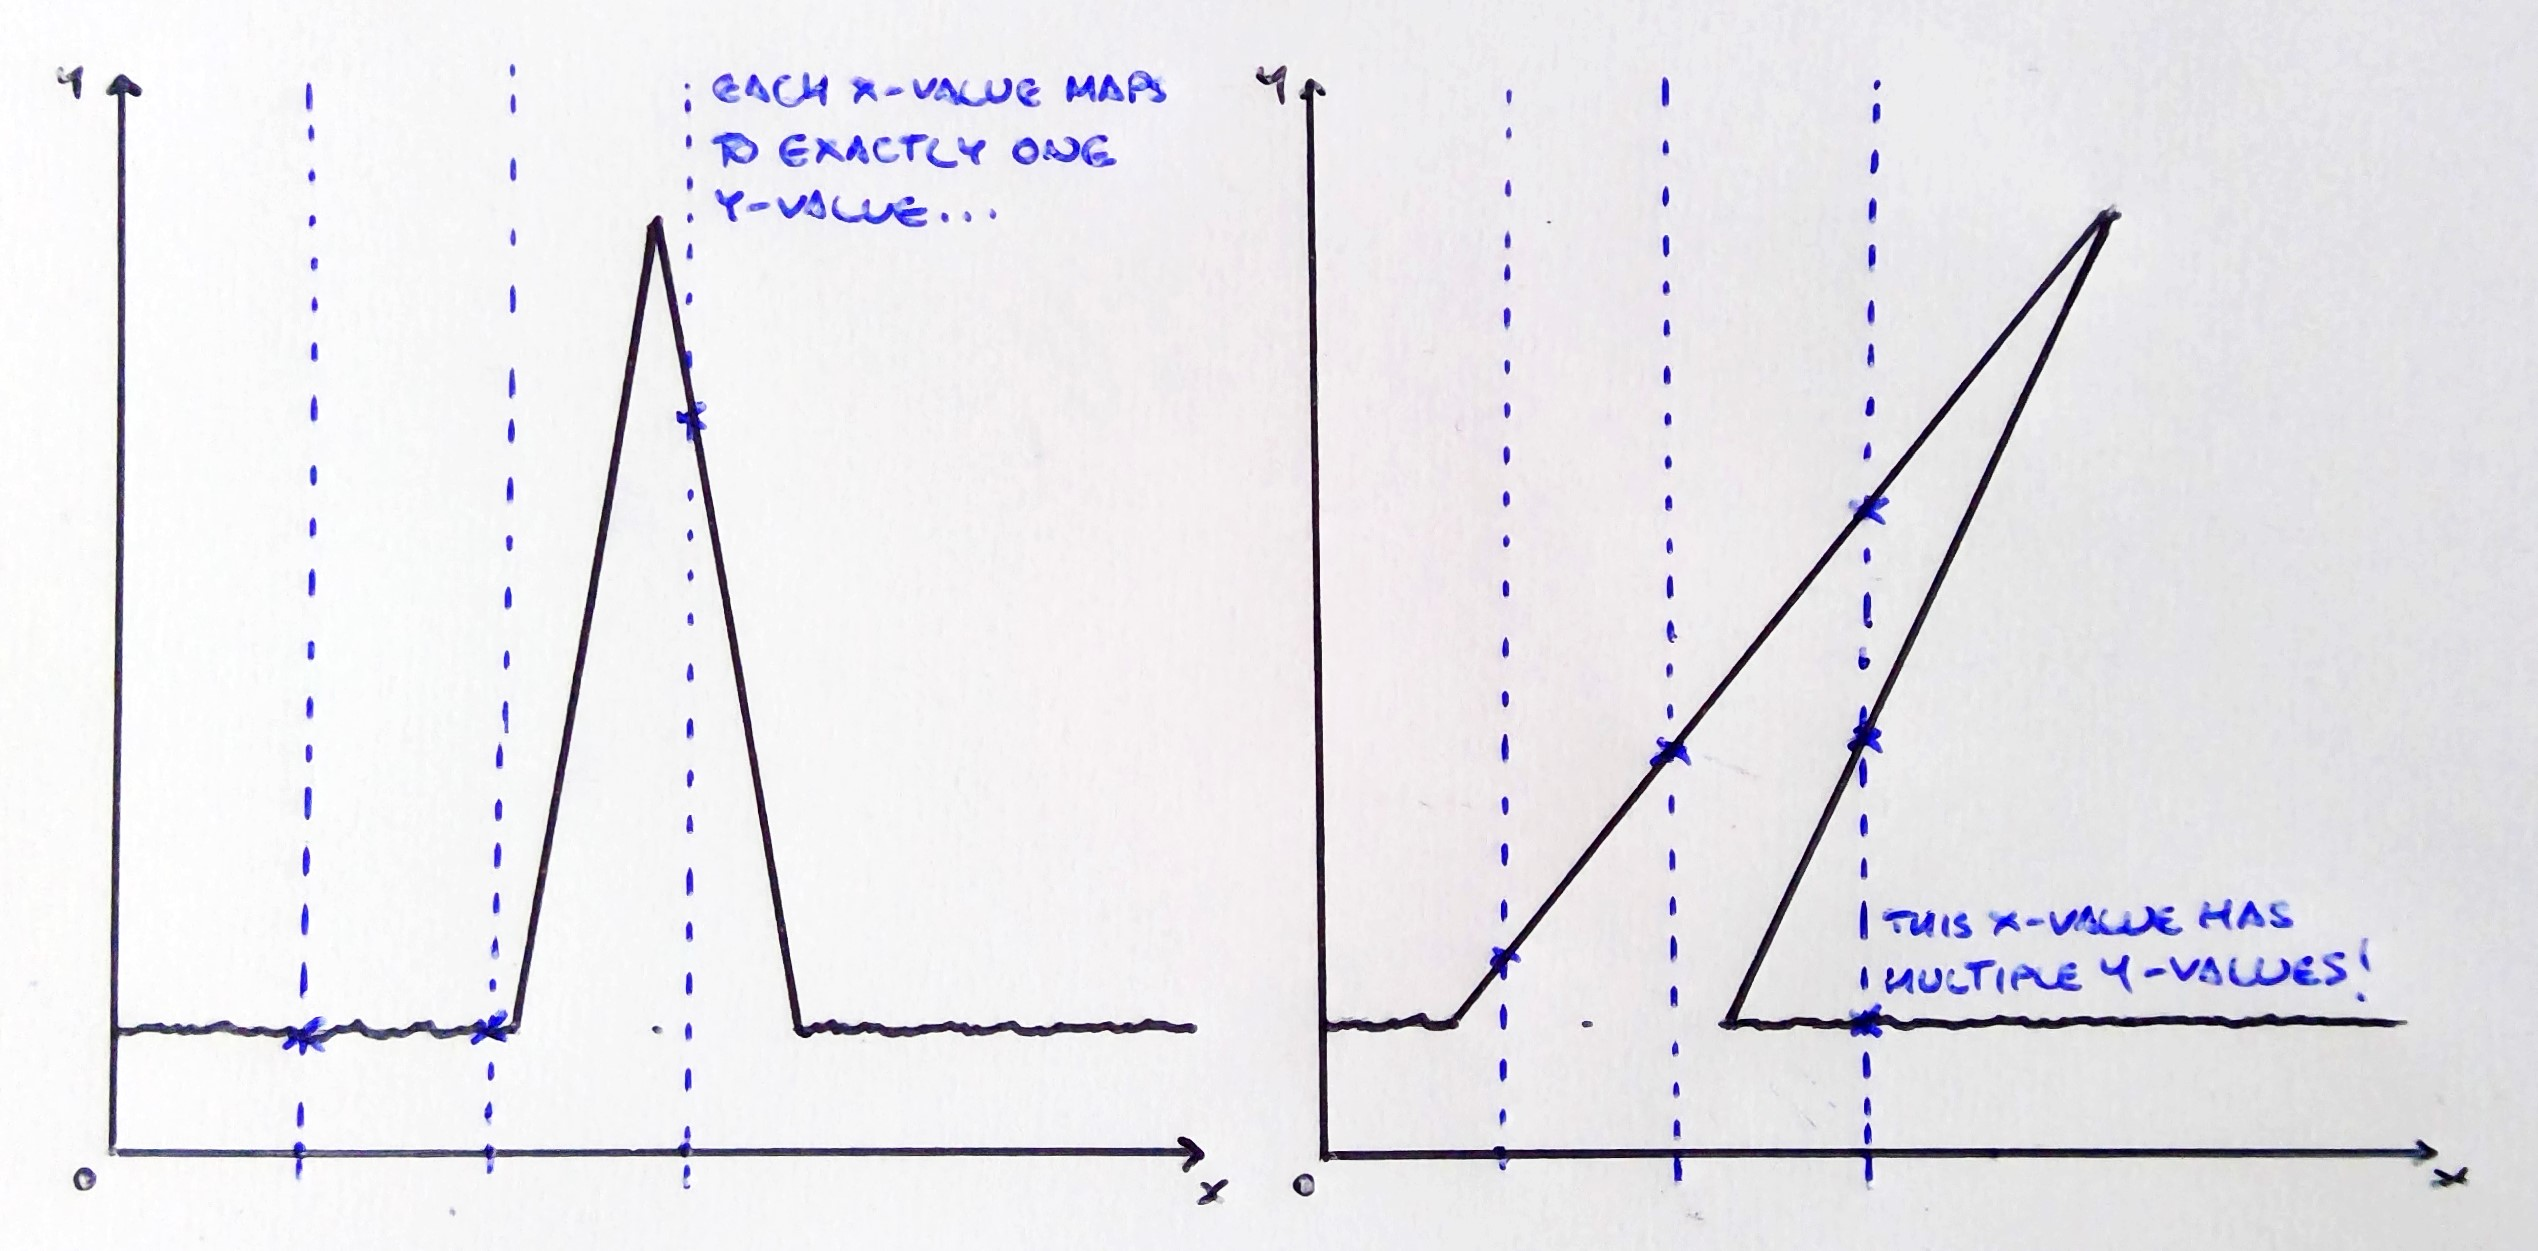
\includegraphics[width=0.9\textwidth]{Concave Terrain}
\caption{Two sketches of \textit{Untitled}'s thorny terrain; though the former can be generated by a height map, the latter is concave.}
\label{Concave Terrain}
\end{figure}

\vspace{5pt}\noindent
Consider the two dimensional analogue here: how might one construct the bounding curve of a (potentially concave, or even disconnected) area? \footnote{This could equally be an $n \times m$ grid; keeping the dimensions the same is just `neater'.}

$$f(x,y) = \min\left(\left(x-0.5\right)^2+\left(y-0.5\right)^2,4\left(\left(x-0.25\right)^2+\left(y-0.75\right)^2\right)\right),$$
describing two overlapping circles.

\begin{figure}[h]
\centering
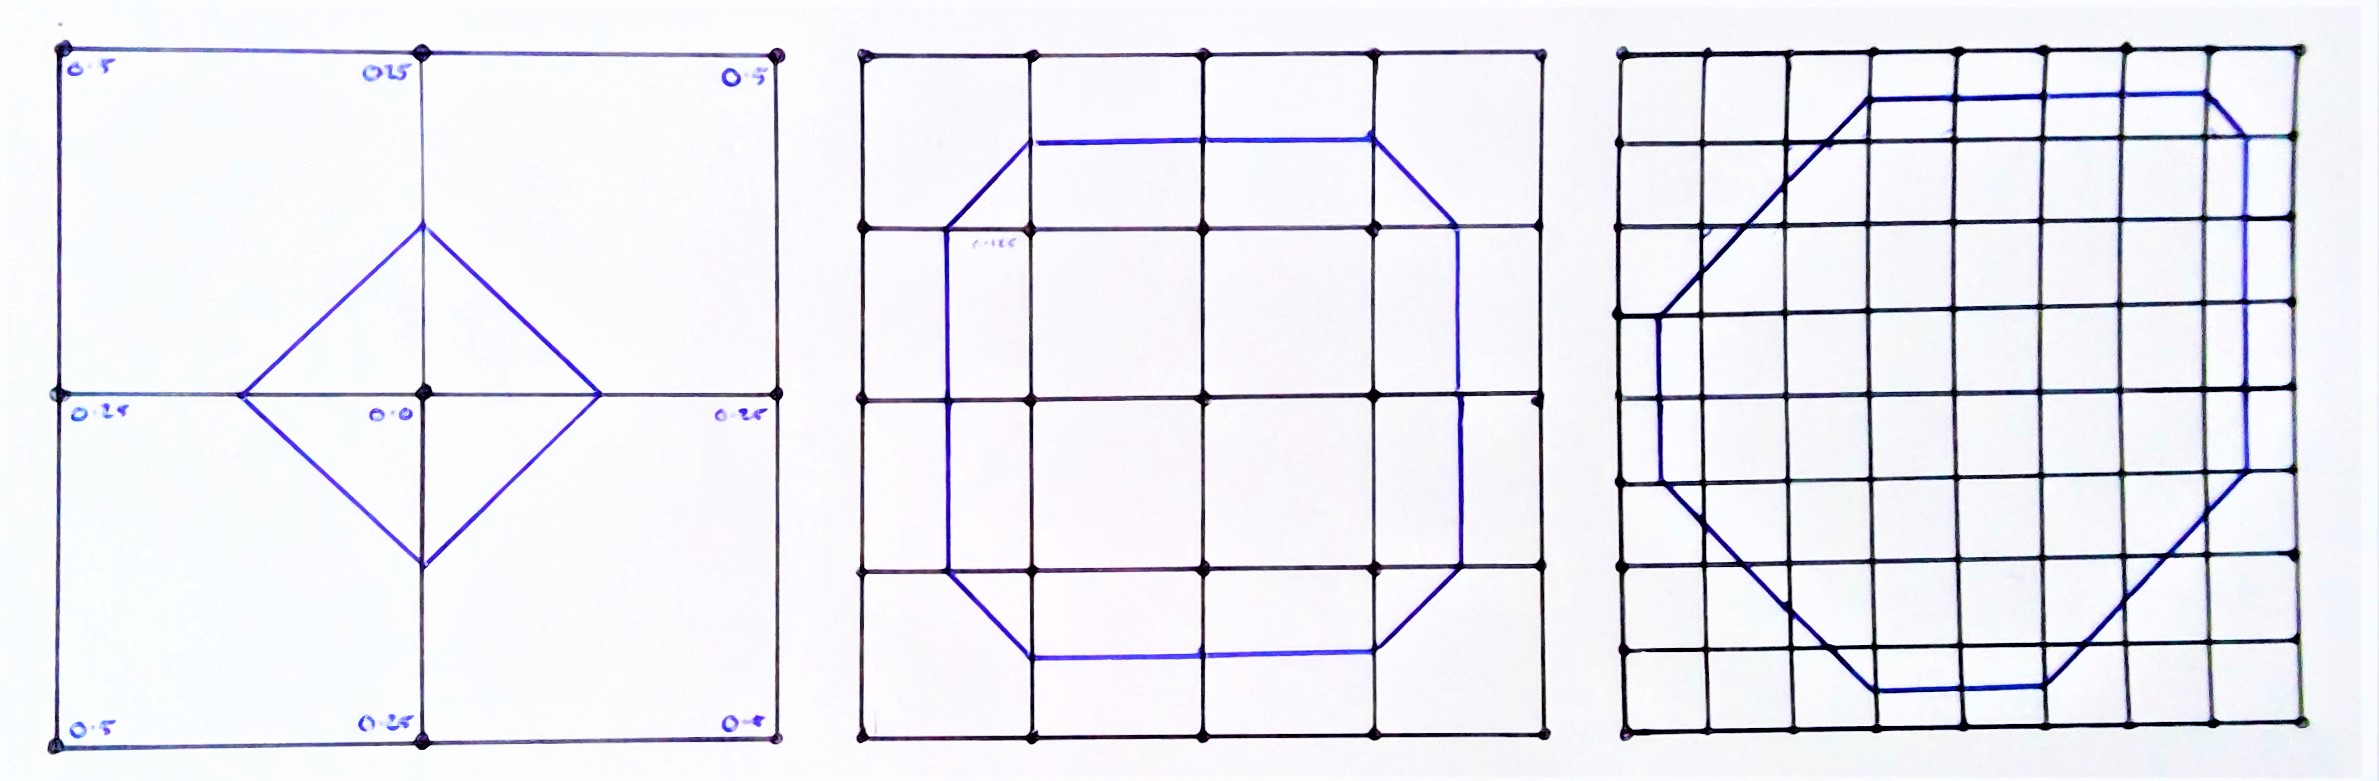
\includegraphics[width=0.9\textwidth]{Marching Squares}
\caption{Bounding curves of $f(x,y) = 0.16$, at increasing levels of granularity.}
\label{Marching Squares}
\end{figure}

\vspace{5pt}\noindent
[Linear interpolation]

\begin{figure}[h]
\centering
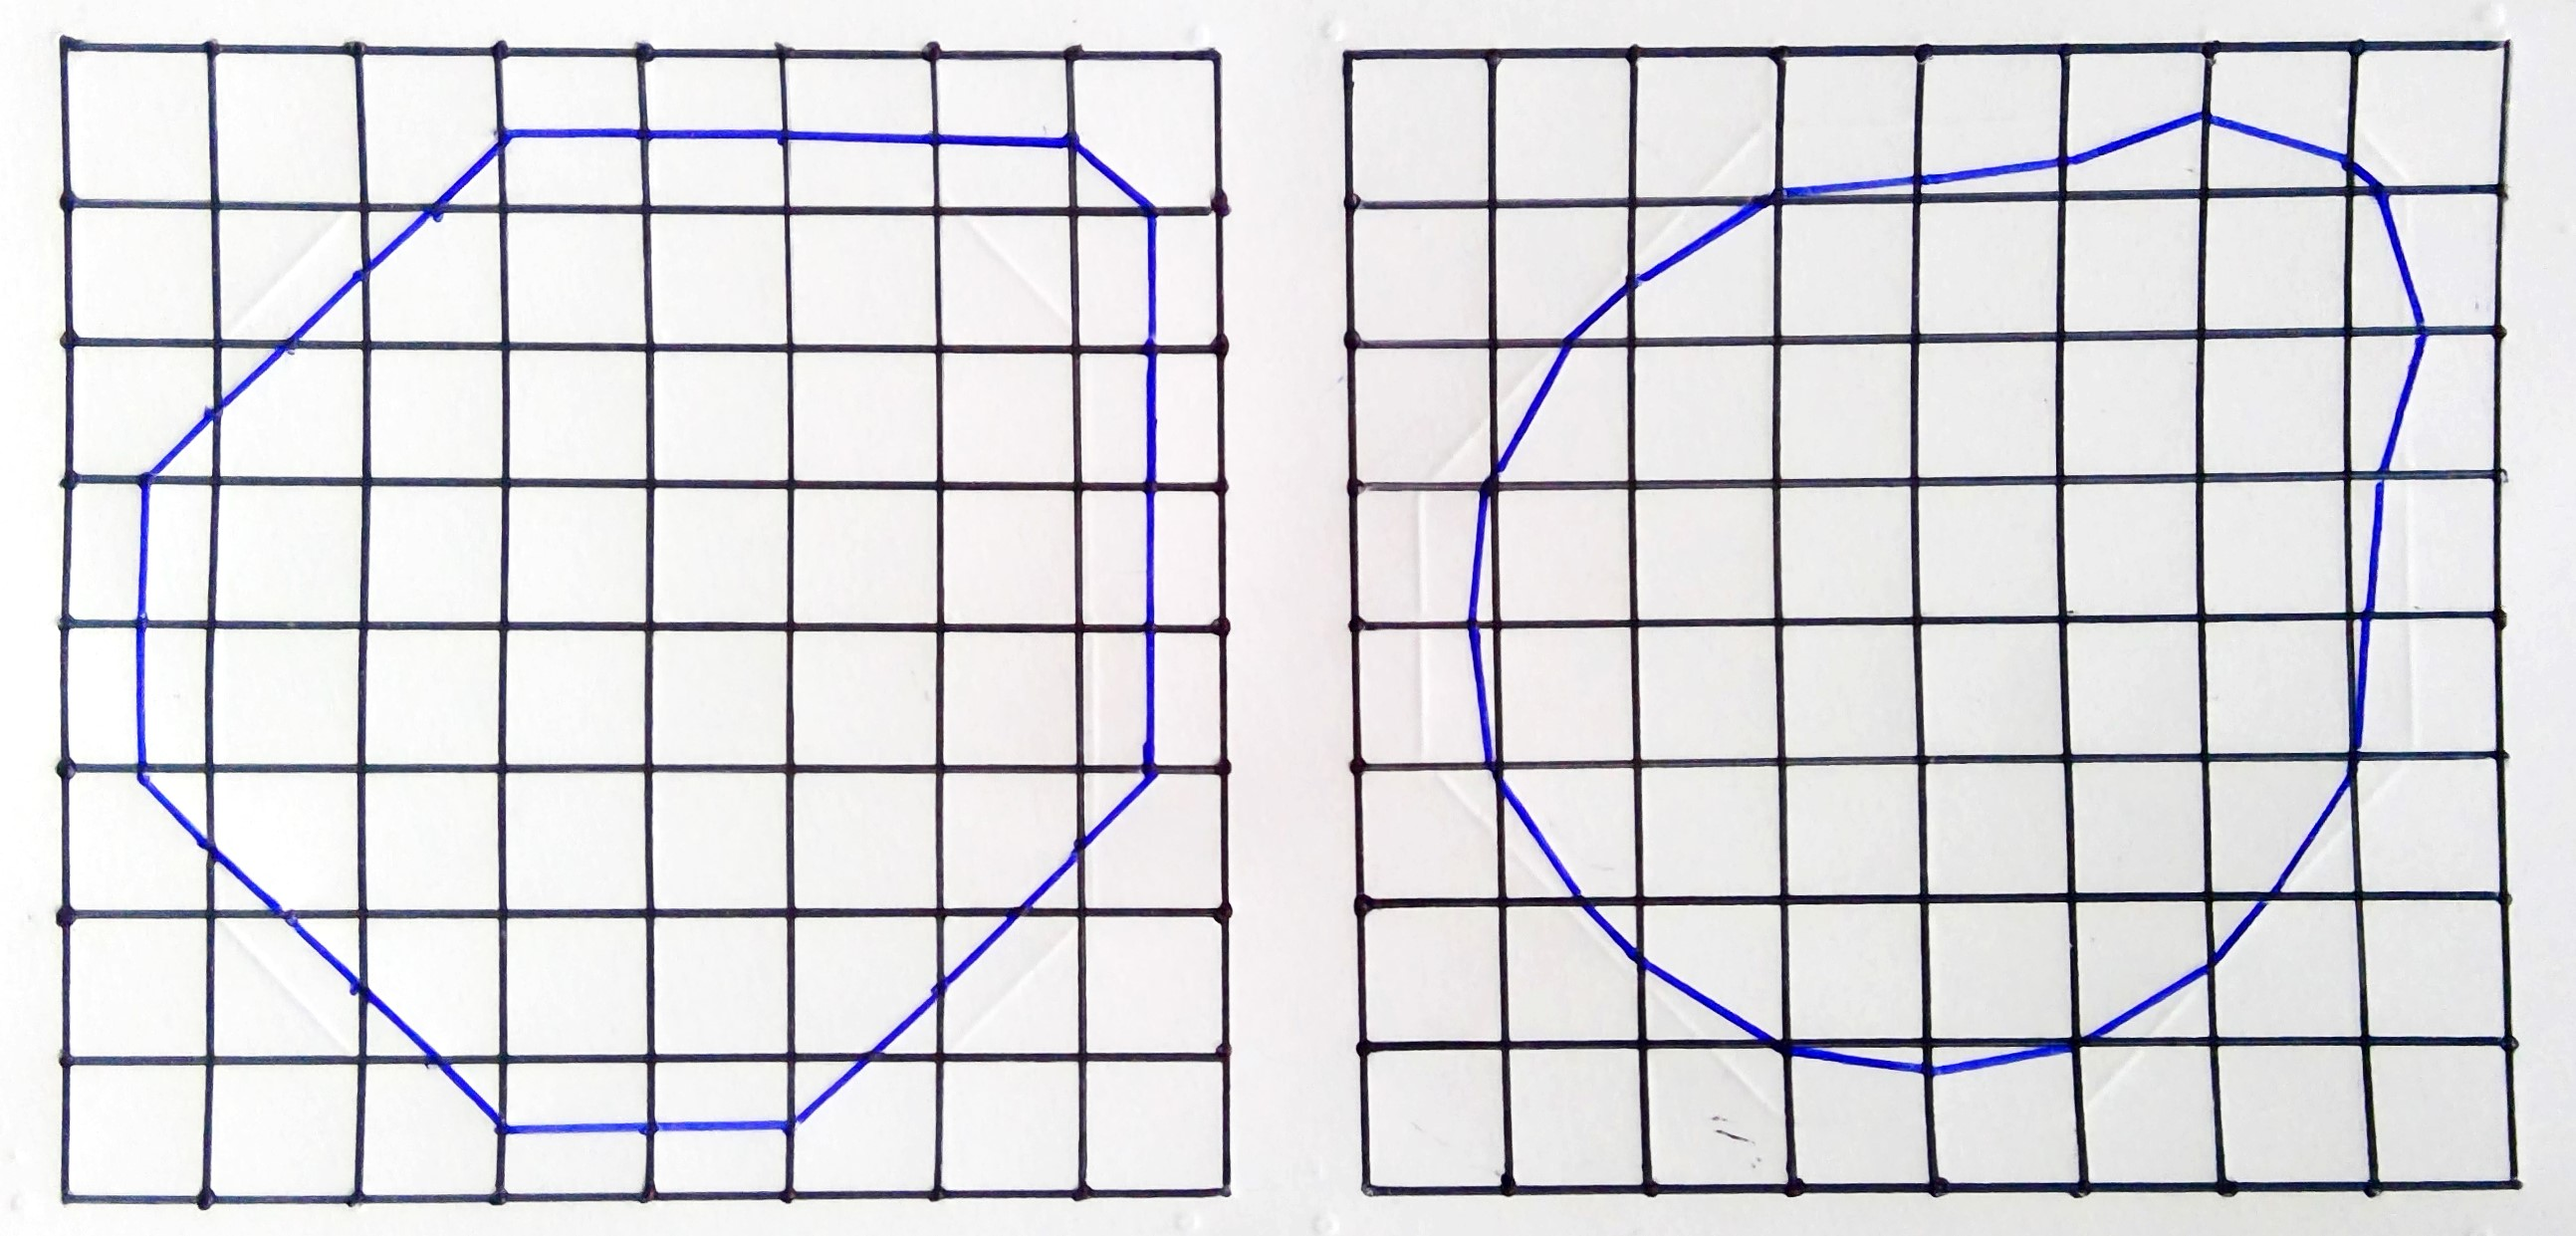
\includegraphics[width=0.9\textwidth]{Interpolated Marching Squares}
\caption{Bounding curves of $f(x,y) = 0.16$, before and after linear intepolation.}
\label{Interpolated Marching Squares}
\end{figure}

\vspace{5pt}\noindent
In much the same way, \textit{Untitled} uses \textit{marching cubes} to generate the bounding surfaces of its 3D volumes. Outside of the expected changes - scalar fields now operate on domain $[0,1]^3$, vertices now have $2^8 = 256$ possible configurations along the edges of each marching cube - this is actually a rather straightforward generalisation.

\vspace{5pt}\noindent
[These are just the broad strokes; nuance to, say, weighing vertex normals correctly]. Definitive... Paul Bourke's \textit{Polygonising a Scalar Field} \citeyearpar{bourkeMarchingCubes} remains the definitive source on the matter. %... [mention marching tetrahedra? While X, marching cubes have been perfectly adequate for the purposes set out below... save this for the evaluation!].

\subsubsection{Case Study: Hexes}

Having . 3D fields are inherently , yet these are essential to carving out \textit{Untitled}'s landscape.

\vspace{5pt}\noindent
Even a blank hex tile comes with som nuance. [Use of noise...]

\vspace{5pt}\noindent
[Bounding hexagonal prism... As much as flat faces are antithetical to marching cubes (if they run parallel to the grid, then... can't interpolate? notice that interpolation doesn't account for the degenerate case where two adjacent gridpoints are equal)...] 

\subsubsection{Case Study: Landmarks}

\subsection{Procedural Screen Textures}\label{Procedural Screen Textures} % TECHNIQUE: L-systems...

The post-processing in \textit{Untitled} is, in one sense, rather simple. The `stress vignette,' for instance, calls only two renders-to-texture on every frame: the board itself, and an alpha map of blood vessels that sprout from the edges of the screen. As striking as the final effect is, \texttt{vignette\_ps.hlsl} is surprisingly straightforward in blending the textures into a single, pulsing eye strain overlay; far more deserving of further discussion is how the blood vessels themselves are generated.

\vspace{5pt}\noindent
In formal languages, a grammar is a tuple $G = (N,\Sigma,P,\omega_0)$. This contains two disjoint sets of symbols: nonterminals $A, B, \dots \in N$, and terminals $a, b, \dots \in \Sigma$. The production rules in $P$ map nonterminals to strings $\alpha, \beta, \dots \in (N\cup\Sigma)^*$; applied recursively to the axiom $\omega_0 \in (N\cup\Sigma)^*$, these rules can produce increasingly complex \textit{sentences} of terminals and/or nonterminals.\footnote{In mathematical literature, $
\omega_0 \in N$ \citep*{hopcroftFormalLanguages}, but \textit{Untitled} takes an informal approach.}

\vspace{5pt}\noindent
The Chomsky hierarchy \citep{chomskyHierarchy} % NB: Is this *strictly* true?
classifies grammars by their production rules:
\begin{enumerate}[label=,itemsep=0em]
\item \textit{Type-3}. \textit{Regular grammars} map $A \mapsto a$ or $A \mapsto aB$.
\item \textit{Type-2}. \textit{Context-free grammars} map $A \mapsto \alpha$.
\item \textit{Type-1}. \textit{Context-sensitive grammars} $\alpha A\beta \mapsto \alpha\gamma\beta$.
\item \textit{Type-0}. \textit{Unrestricted grammars} map $\alpha \mapsto \beta$, where $\alpha$ is non-empty.
\end{enumerate}
Note that all Type-3 grammars are also Type-2, all Type-2 grammars also Type-1, and so on.

\vspace{5pt}\noindent
Suppose, for example, that $N = \{F, G\}$, $\Sigma = \{+, -\}$, $P = \{F \mapsto F+G, G \mapsto F-G\}$, $\omega_0 = F$.
Letting $\omega_n$ denote the sentences generated by applying the production rules $n$ times, it follows that
$$\begin{matrix*}[l]
\omega_1 &= &F+G, \\
\omega_2 &= &F+G+F-G, \\
\omega_3 &= &F+G+F-G+F+G-F-G, \\
\omega_4 &= &F+G+F-G+F+G-F-G+F+G+F-G-F+G-F-G, \;\; \cdots.
\end{matrix*}$$

\vspace{5pt}\noindent
While these defintions are rather abstract, \citet{lindenmayerLSystems} provides a remarkable application. Treating each symbol as an instruction like `go forward' or `turn right', \textit{L-systems} visualise sentences via `turtle graphics'; when those sentences have been generated recursively by a grammar, the line drawings inherit that same self-similar structure. Consider the above, where reading non-terminals $F$, $G$ as `draw a line while moving one unit forwards,' and terminals $\pm$ as `turn $\pm\, \pi/2$ on the spot,' produces the fractal dragon curves in Figure \ref{Dragon Curves}.

%\vspace{5pt}\noindent
\begin{figure}[h]
\centering
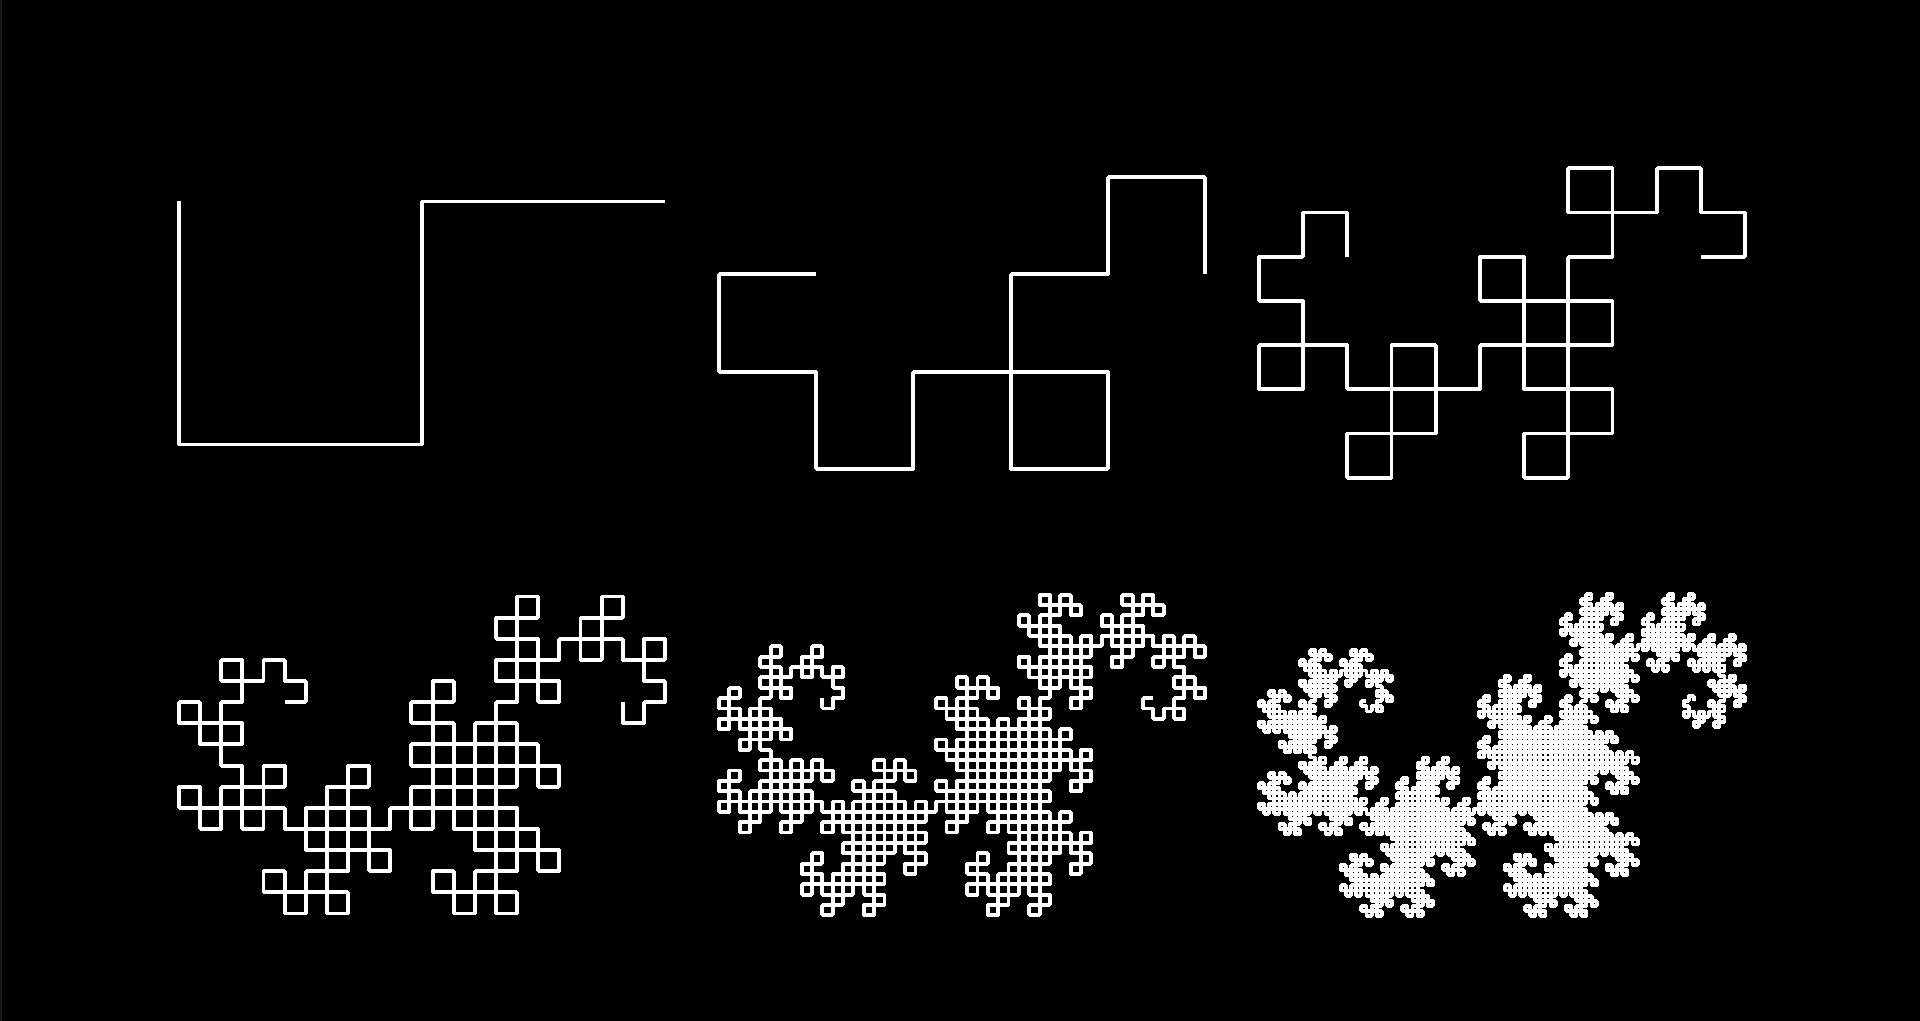
\includegraphics[width=0.66\textwidth]{Dragon Curves}
\caption{Dragon curves, generated by strings $\omega_2, \omega_4, \cdots, \omega_{12}$.}
\label{Dragon Curves}
\end{figure}

\vspace{5pt}\noindent
While L-systems are most common in the modelling of 3D plants and other branching structures \citep{prusinkiewiczAlgorithmicBeauty}, \textit{Untitled} only uses them to generate 2D alpha maps. Moreover, it restricts its attention to L-systems paired with context-free grammars.

\subsubsection{Case Study: Runes}

Parametric L-systems \citep{hananParametricLSystems} exist as a generalisation of the above. [theory].

\vspace{5pt}\noindent
The modules in \textit{Untitled}, then, track three . More than anything, this offers a certain clarity of code - at least from a 

\vspace{5pt}\noindent
[Example: various geometric runes!].

\subsubsection{Case Study: Blood Vessels} % Include post-processing!

\citet{zamirArterialBranchingLSystems}, meanwhile, uses parametric L-systems to visualise the bifurcation of blood vessels. Suppose a branch with length $l$, width $w$ bifurcates into two branches $M$ and $m$, such that $l_M \geq l_m$. Defining the \textit{asymmetry ratio} $\alpha = l_m/l_M$, it follows that
$$l_M = \frac{l}{\left(1+\alpha^3\right)^{1/3}}, \;\; l_m = \frac{\alpha\cdot l}{\left(1+\alpha^3\right)^{1/3}}, \;\; w_M = \frac{w}{\left(1+\alpha^3\right)^{1/3}}, \;\; w_m = \frac{\alpha\cdot w}{\left(1+\alpha^3\right)^{1/3}}.$$
Furthermore, the branches diverge from their parent at angles
$$\theta_M = \arccos\left(\frac{\left(1+\alpha^3\right)^{4/3}+1-\alpha^4}{2\left(1+\alpha^3\right)^{2/3}}\right), \;\; \theta_m = \arccos\left(\frac{\left(1+\alpha^3\right)^{4/3}+\alpha^4-1}{2\alpha^2\left(1+\alpha^3\right)^{2/3}}\right).$$
\textit{Untitled}'s framework is therefore capable of reproducing \citeauthor{zamirArterialBranchingLSystems}'s results (see Figure \ref{Zamir Branching}), using an L-system with the single production rule:  
$$\mathbf{C}(l,w,\theta) \mapsto \mathbf{X}(l,w,\theta)[\mathbf{C}(l_M,w_M,\theta+\theta_M)]\mathbf{C}(l_m,w_m,\theta-\theta_m).$$

%\vspace{5pt}\noindent
\begin{figure}[h]
\centering
%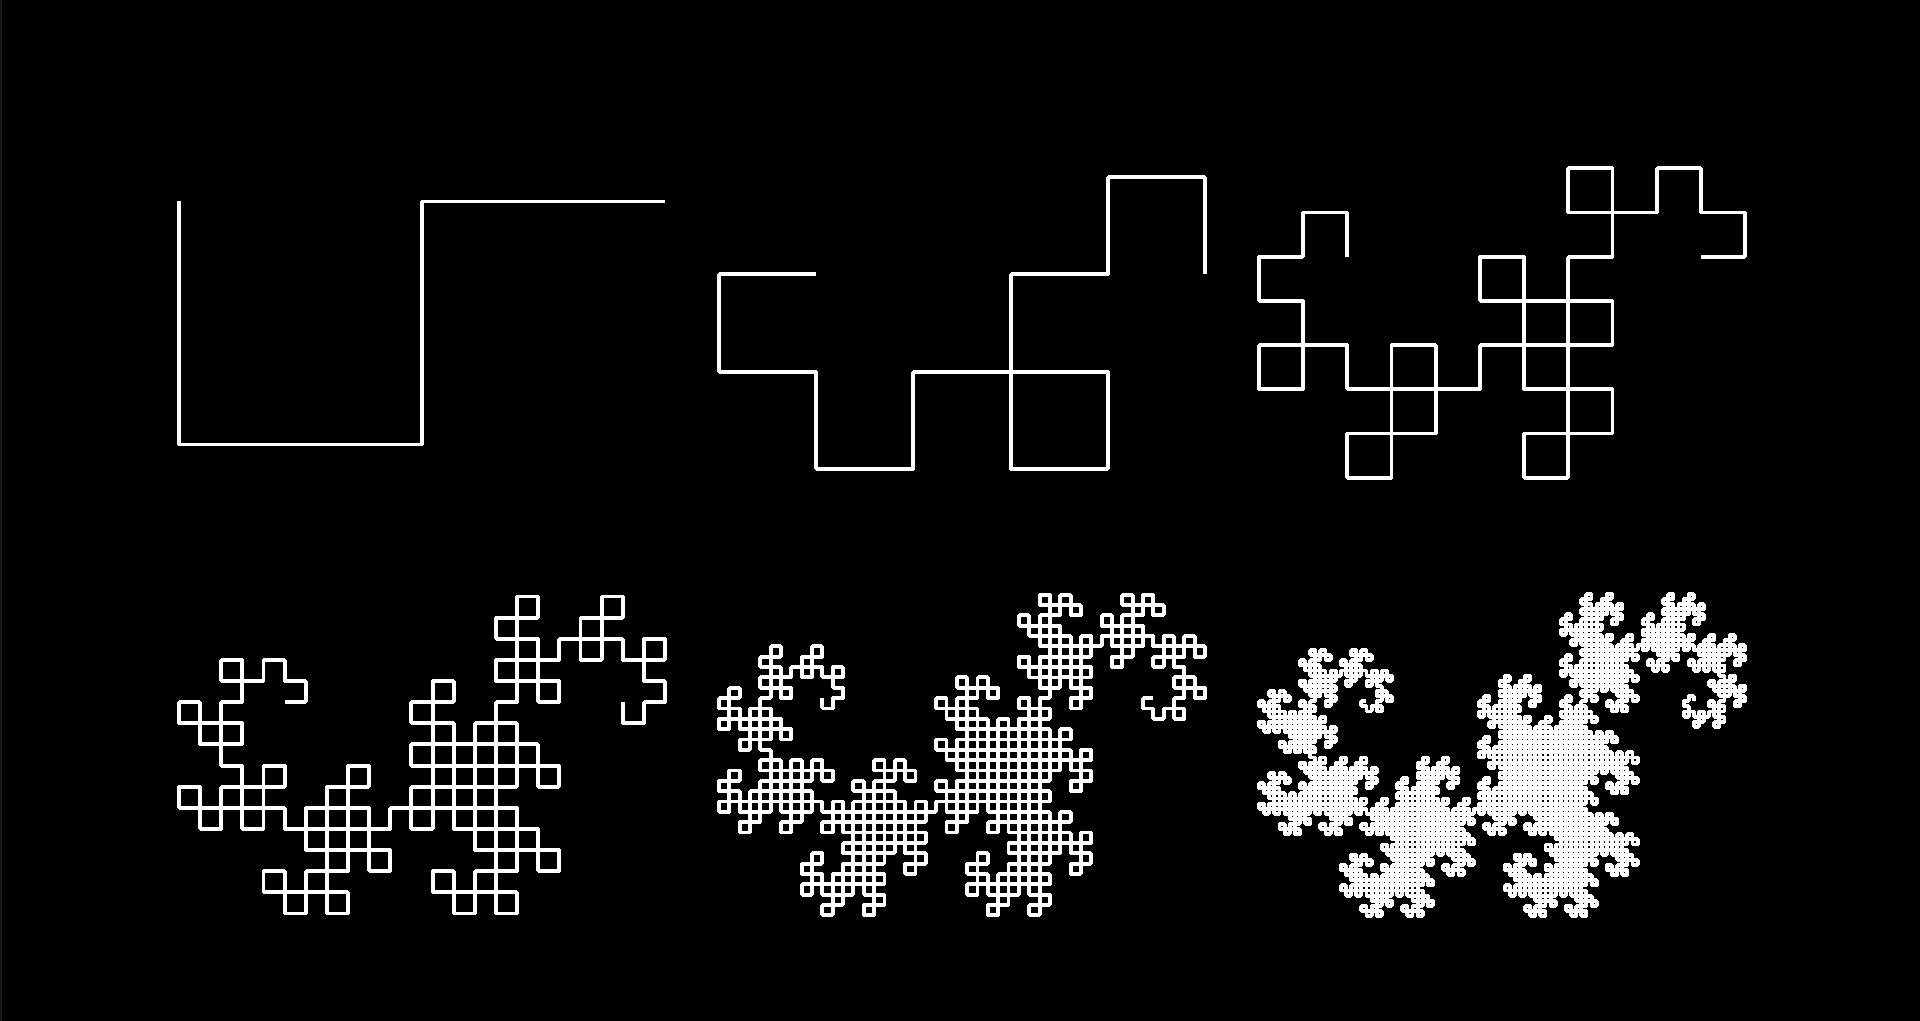
\includegraphics[width=0.66\textwidth]{Dragon Curves}
\caption{\citeauthor{zamirArterialBranchingLSystems}'s model of arterial branching, with asymmetry ratios $\alpha = 1.0, 0.8, \cdots, 0.2$.}
\label{Zamir Branching}
\end{figure}

%\vspace{5pt}\noindent
%$$\begin{matrix*}[l]
%\mathbf{C} &\mapsto &\mathbf{X}[+\mathbf{C}]-\mathbf{C} \\
%\mathbf{X} &\mapsto &\mathbf{X}\mathbf{X}
%\end{matrix*}$$

%\vspace{5pt}\noindent
%$$\begin{matrix*}[l]
%\mathbf{C}, \\
%\mathbf{X}[+\mathbf{C}]-\mathbf{C}, \\
%\mathbf{X}\mathbf{X}[+\mathbf{X}[+\mathbf{C}]-\mathbf{C}]-\mathbf{X}[+\mathbf{C}]-\mathbf{C}, \\
%\mathbf{X}\mathbf{X}\mathbf{X}\mathbf{X}[+\mathbf{X}\mathbf{X}[+\mathbf{X}[+\mathbf{C}]-\mathbf{C}]-\mathbf{X}[+\mathbf{C}]-\mathbf{C}]-\mathbf{X}\mathbf{X}[+\mathbf{X}[+\mathbf{C}]-\mathbf{C}]-\mathbf{X}[+\mathbf{C}]-\mathbf{C}, \;\; \cdots
%\end{matrix*}$$

%\vspace{5pt}\noindent
%$$\begin{matrix*}[l]
%\mathbf{C}(l,w,\theta) &\xmapsto[0.4]{} &\mathbf{X}(l,w,\theta)[\mathbf{C}(l_M,w_M,\theta+\theta_M)]\mathbf{C}(l_m,w_m,\theta-\theta_m) \\
%\mathbf{C}(l,w,\theta) &\xmapsto[0.4]{} &\mathbf{X}(l,w,\theta)[\mathbf{C}(l_m,w_m,\theta+\theta_m)]\mathbf{C}(l_M,w_M,\theta-\theta_M) \\
%\mathbf{C}(l,w,\theta) &\xmapsto[0.2]{} &\mathbf{X}(l,w,\theta)\mathbf{C}(l,w,\theta) \\
%\end{matrix*}$$

\vspace{5pt}\noindent
\citet{liuSimulationBloodVessels} expand on this by introducing a stochastic component - that is to say, they allow [a more random structure]. \textit{Untitled} incorporates such randomness into its own rules for blood vessels:
$$\begin{matrix*}[l]
\mathbf{C}(l,w,\theta) &\xmapsto[0.4]{} &\mathbf{X}(l,w,\theta)[\mathbf{L}(l_M,w_M,\theta+\theta_M)]\mathbf{R}(l_m,w_m,\theta-\theta_m) \\
\mathbf{C}(l,w,\theta) &\xmapsto[0.4]{} &\mathbf{X}(l,w,\theta)[\mathbf{L}(l_m,w_m,\theta+\theta_m)]\mathbf{R}(l_M,w_M,\theta-\theta_M) \\
\mathbf{C}(l,w,\theta) &\xmapsto[0.2]{} &\mathbf{X}(l,w,\theta)\mathbf{C}(l,w,\theta) \\
& & \\
\mathbf{L}(l,w,\theta) &\xmapsto[1.0]{} &\mathbf{X}(l,w,\theta)\mathbf{C}(l_M,w_M,\theta-\theta_M) \\
& & \\
\mathbf{R}(l,w,\theta) &\xmapsto[1.0]{} &\mathbf{X}(l,w,\theta)\mathbf{C}(l_M,w_M,\theta+\theta_M)
\end{matrix*}$$
These describe a capillary with a 40\% chance of bifurcating with branch $M$ tacking clockwise, a 40\% chance of bifurcating with $M$ tacking anticlockwise, and a 20\% chance of extending forwards without any branching. The determinstic production rules on $\mathbf{L}$, $\mathbf{R}$ provide course correction, guaranteeing the [...]; further informal tweaks can be found in the \texttt{LBloodVessel} class, all intended to get the final look of the L-systems `right' (see Figure [reference]). 

\vspace{5pt}\noindent
[Figure of blood vessels in isolation]

\vspace{5pt}\noindent
[Discussion of animation (and the shortcomings thereof)...]

\vspace{5pt}\noindent
[Figure of final render]

\subsection{Procedural Narrative} % TECHNIQUE: 'Improv-lite' text generation...

\textit{Untitled} was originally conceived as a showcase of procedural text generation, an application of [authored X] towards interactive fiction. 

\subsubsection{Grammars}

Given their origin in linguistics, it is perhaps unsurprising that grammars (see Section \ref{Procedural Screen Textures}) are of use in the field of procedural narrative - \textit{Tracery} \citep{comptonTracery} being the prime example. From a mathematical perspective, this is a stochastic, context-free grammar, with uniformly-distributed production rules for each non-terminal; it iterates a given axiom until all non-terminals (demarcated by \texttt{\#HASHTAG\#} delimiters) have been replaced. To bemoan the generator as better suited to Twitter bots than immersive storytelling is to misunderstand its design. \citeauthor{comptonTracery} present a lightweight tool that is left \textit{deliberately} narrow, intended for ease-of-use amongst even the most fledgling authors.

\vspace{5pt}\noindent
More substantial works, then, adapt \textit{Tracery}'s grammar-based approach to their own specifications. In \textit{The Annals of the Parrigues}, \citeauthor{shortParrigues} sets out the need for a consistent generator, one that ``defines any facts about the world that aren’t already defined at the moment of generation'' (\citeyear{shortParrigues}, p. 83). \textit{Voyageur} \citep{diasVoyageur} attaches weightings to the distributions of production rules \citep{diasVoyageurDescriptions}. Produceral storytelling is an art form; as much as \textit{Untitled} wears these influences on its sleeve, to try and consolidate these into an `optimal', one-size-fits-all generator would be missing the point. This project therefore uses an implementation of \textit{Tracery} with a couple of custom modifications tailored to its own needs.

\paragraph{Recency} [Clear, one sentence goal: avoid unnecessary repetition with recency].\footnote{\textit{Improv}, the generator for \textit{Voyageur}, calls this same quality `dryness'.} \textit{Untitled} defines this by rank: given a non-terminal with $N$ possible production rules, the most recently used rule is will have a recency of $N-1$, the second most recent $N-2$, and so on down to the rule that has been used longest ago (or indeed, never been used), with recency $0$. Though it [does not consider the actual time interval between these uses, nor the \textit{second} most ], this metric is already enough to achieve the desired effect \citep{kazemiSimpleProceduralGeneration}.

\vspace{5pt}\noindent
[Second paragraph: how does this affect weighting?] $p^{n/(N-1)}$, such that (all other weightings being equal), the most recently used rule (with $n = N-1$) will be $p$ times as likely as the least recent ($n = 0$).\footnote{The same string \texttt{alpha} might replace two different non-terminals \texttt{\#A\#}, \texttt{\#B\#}. Recognising these as distinct production rules, the recency with which one was applied to \texttt{\#A\#} has no bearing on when the other is applied to \texttt{\#B\#}, or vice versa.} 

\vspace{5pt}\noindent
Note that [joint recency!].

\paragraph{Characterisation} [Consistency discussion...]

\vspace{5pt}\noindent
This might feel too limited, from a dramatic perspective. For all this effort to [maintain consistency], personality is not immutable; so much of good storytelling relies on character \textit{development}.
Indeed, how does the player feel like they have an impact, if [the grammar doesn't have permission to make changes]? \textit{Untitled} surely requires some sort of override...
%Does this make sense, dramaturgically?

\subsubsection{Content Selection Architectures} \textit{Storylets} \citep{kreminskiStorylets} are [definition].

\vspace{5pt}\noindent
[Though conceptually no different, ... , our `narrative stack'...]
 
\section{Code Organisation}

[...]

\vspace{5pt}\noindent
Section \ref{Features} has been structured [to reflect the two fundamental stages of graphics programming: first implementing frameworks (marching cubes, L-systems), then building tangible objects out of them (terrain hexes, blood vessels)]. \textit{Untitled}'s code is structured accordingly. [Using inheritance...]. [Crucially, little is left exposed in the main \textit{Game.cpp} file...].

%Mention use of `tags' in JSON?

\subsection{Rendering}

\subsection{GUI}

[Include HDRR/bloom here...]

\section{Evaluation}\label{Evaluation}

\subsection{Features}

[Start with marching cubes: successful, but more to do...]

\vspace{5pt}\noindent
[L-systems: far more robust...]

\vspace{5pt}\noindent
To the extent that \textit{Untitled} has any single `special feature', though, it would surely be its approach to procedural storytelling. [...]

\subsection{Code Organisation}

[Position weakness of the storytelling as an \textit{organisational} matter...]

\vspace{5pt}\noindent
[Discuss the broader merits of Section 4, ultimately landing on the value of \textit{internal consistency}.]

\section{Conclusions}

From a more personal perspective, I can't help but feel that \textit{Untitled} shows promise.

\vspace{5pt}\noindent
[Coheres in a way that my CMP502 project absolutely didn't...]. [Furthermore, a better sense of performance] - I might not be happy with the loading times \textit{per se}, but all things considered these advanced graphics techniques will still run on my laptop.

\vspace{5pt}\noindent
Of course, there is a distinction to be drawn between \textit{Untitled}'s functionality as a graphics showcase and as a game. As much as there's a certain level of interactivity on display,\footnote{And likewise, non-interactive features like the fixed, orthographic camera carry some level of intentionality...} [Perils of interactive narrative].

\vspace{5pt}\noindent
[What/how would I go about cannibalising this? Screen shader first/hexes... narrative much more an early experiment in structuring content selection architectures/context-sensitive grammars...]

\bibliographystyle{agsm}
\bibliography{../../Bibliography/Bibliography}
\addcontentsline{toc}{section}{References}
\end{flushleft}
\end{document}
